\section{Hardware}
  Für die technische Umsetzung werden eine Reihe von Komponenten verwendet.

  \subsection{Raspberry Pi 3}
  
    % image of the raspberry pi - source: http://www.raspberrypi.org
    \begin{minipage}{\columnwidth}
      \makeatletter
      \def\@captype{figure}
      \makeatother
      \centering
      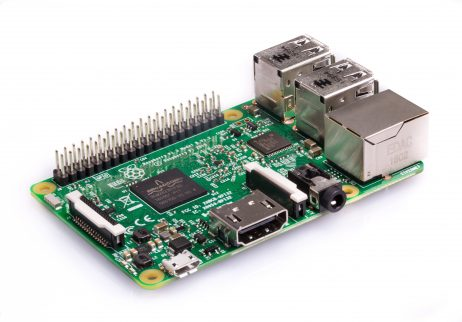
\includegraphics[width=0.6\linewidth]{images/hw_raspberrypi3.jpg}
      \caption{Raspberry Pi 3 Model B}
      \label{fig:img-hw-01}
    \end{minipage}
    \vspace{1cm}

    \noindent
    Das Herzstück des Projekts bildet ein Raspberry Pi 3 Model B. Ausgestattet
    ist dieser Mini-PC neben den üblichen Schnittstellen mit drei Elementen, die
    für das Vorhaben essentiell sind: Einem Wifi Modul, einem Ethernet-Port und
    allem einem GPIO Header mit reichlich freien Pins.\\
    \ \\
    Als Betriebssystem nutzt der Raspberry Pi das hauseigene Debian Derivat
    Raspbian. \\

  \subsection{Motorcontroller}

    % image of the motor and servo controller module  - source: https://www.makerlab-electronics.com
    \begin{minipage}{\columnwidth}
      \makeatletter
      \def\@captype{figure}
      \makeatother
      \centering
      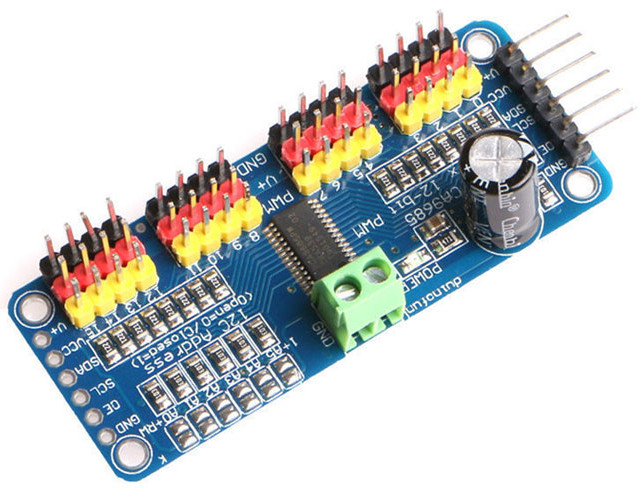
\includegraphics[width=0.6\linewidth]{images/hw_pca9685.jpg}
      \caption{PCA9685 Controller Modul}
      \label{fig:img-hw-02}
    \end{minipage}
    \vspace{1cm}

    \noindent
    Der Fahrtenregler des Motors für den Antrieb und der Servo für die Lenkung
    des RC Fahrzeugs werden über das PCA9685 Controller Modul mittels
    Pulsweitenmodulation angesprochen. Die Implementierung selbst ist
    glücklicherweise bereits durch eine offene Python Bibliothek (siehe Tab.
    \ref{tab:sw-01}) verfügbar. 
  
  \subsection{Raspberry Pi Camera Module}
    % image of the camera module - source: https://www.raspberrypi.org
    \begin{minipage}{\columnwidth}
      \makeatletter
      \def\@captype{figure}
      \makeatother
      \centering
      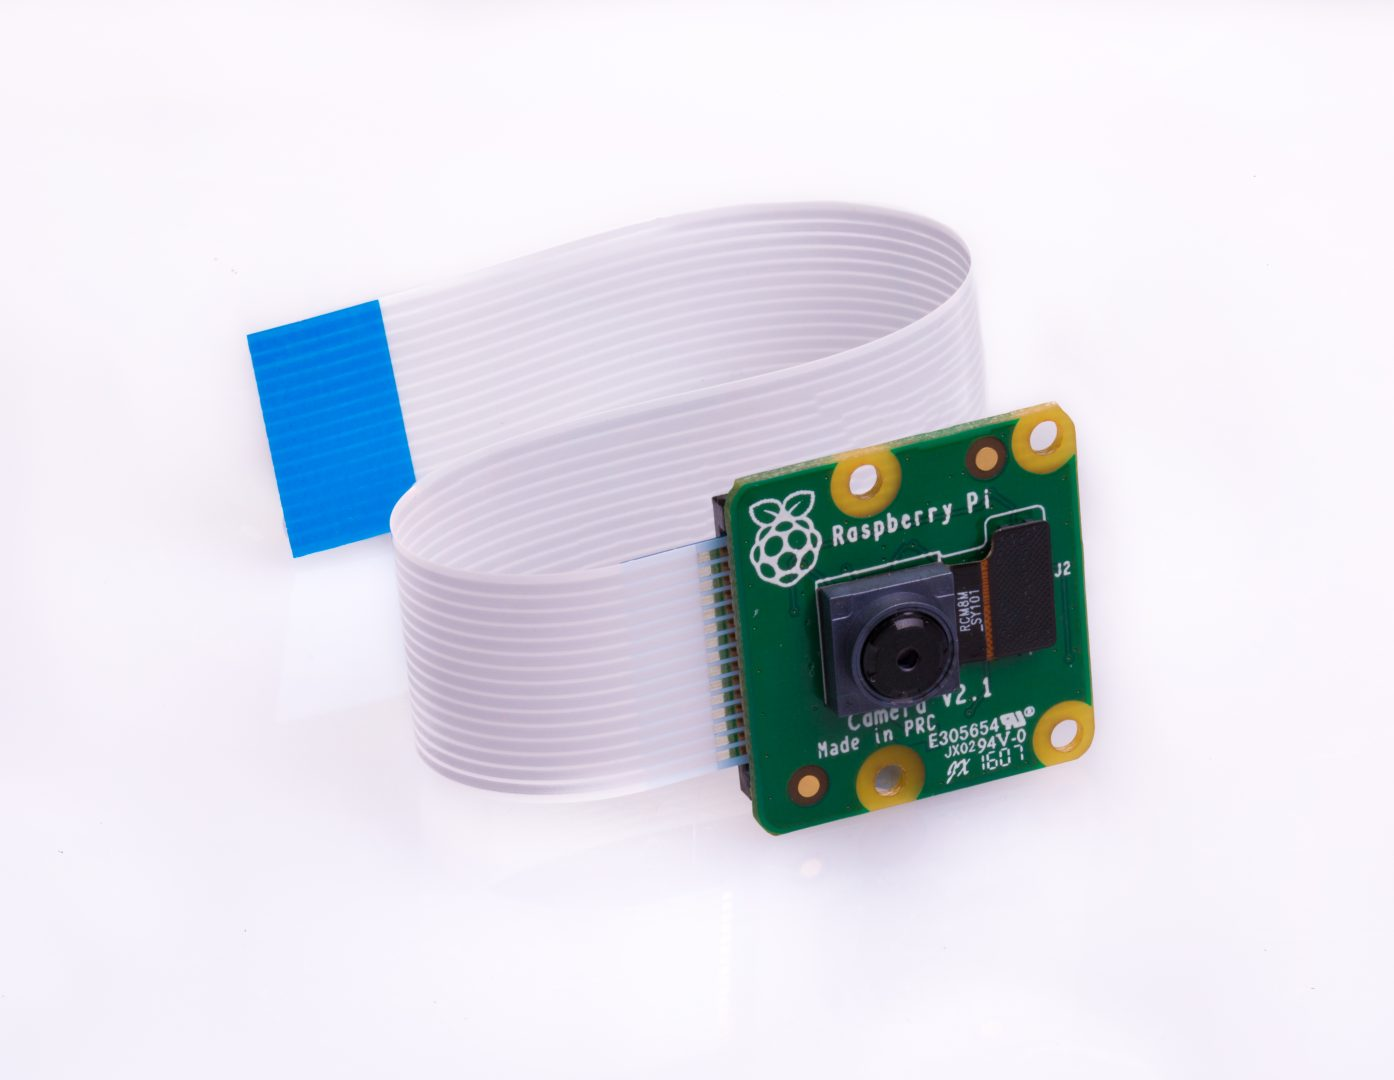
\includegraphics[width=0.6\linewidth]{images/hw_picam.jpg}
      \caption{Camera Module V2}
      \label{fig:img-hw-03}
    \end{minipage}
    \vspace{1cm}

    \noindent
    Das Sehen ermöglicht das eingesetzte Raspberry Pi Kameramodul, welches über
    einen speziell am Raspberry Pi vorhandenen Kameraanschluss. Verbaut ist
    ein Sony IMX219 8-Megapixel Sensor der ebenfalls direkt über vorhandene
    Python Bibliotheken performant und resourcenschonend ausgelesen werden kann.

  \subsection{Ultraschallsensor}

    % image of ultrasonic sensor module  - source: https://www.makerfabs.com 
    \begin{figure}[H]
    \center
    \begin{subfigure}{.5\textwidth}
      \centering
      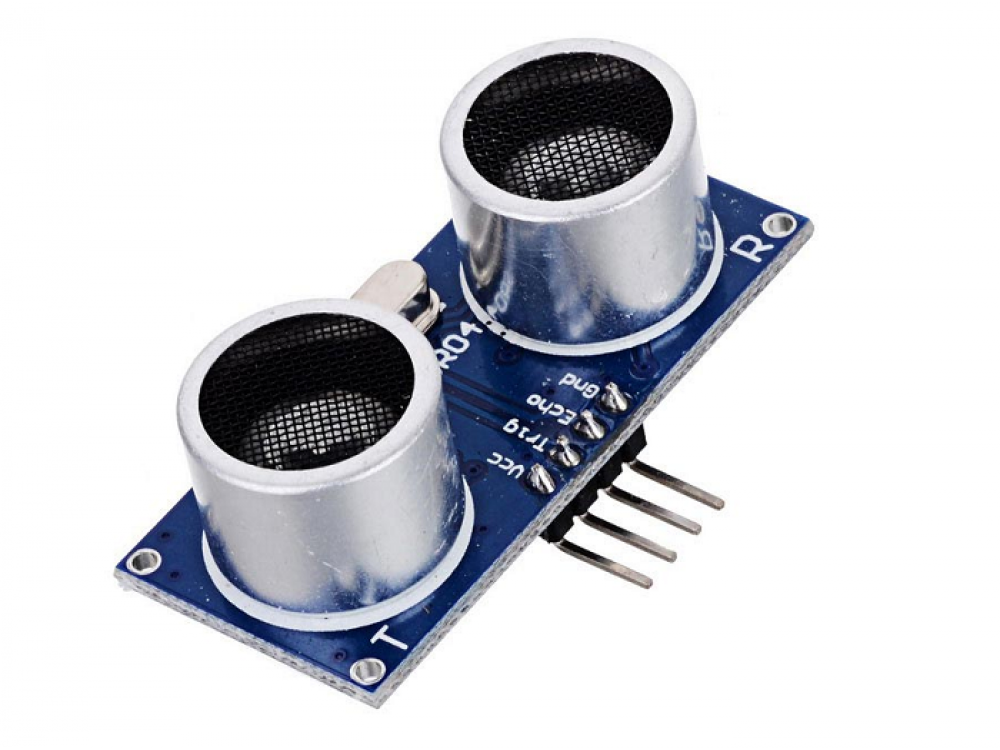
\includegraphics[width=.8\linewidth]{images/hw_hcsr04_01.png}
    \end{subfigure}%
    \begin{subfigure}{.5\textwidth}
      \centering
      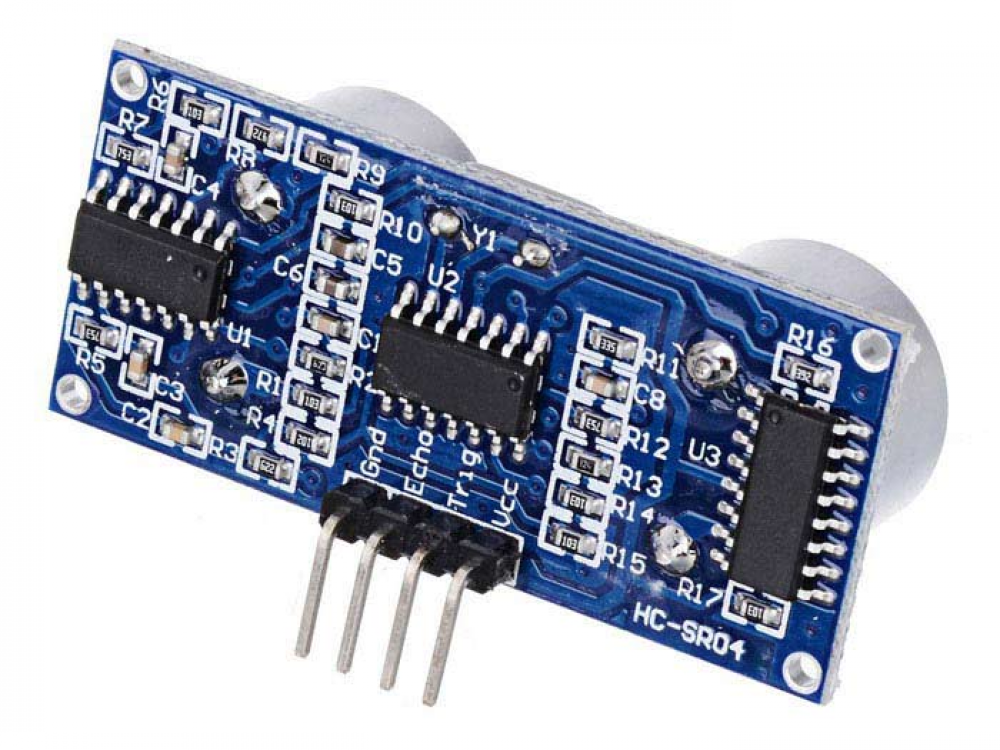
\includegraphics[width=.8\linewidth]{images/hw_hcsr04_02.png}
    \end{subfigure}
      \caption{HC-SR04 Sensor Modul}
      \label{fig:img-hw-04}
    \end{figure}
    \vspace{1cm}
    Im Falle eines anstehenden Frontalzusammenstoßes mit einer Wand oder einem
    anderen größeren Hindernis, soll zusätzlich zur Kamera vorne am Fahrzeug ein
    Ultraschallsensor angebracht werden, der unmittelbare Hindernisse melden
    kann. Hier kommt der HC-SR04 zum Einsatz. Für die Abstandsmessung sendet
    dieser in regelmäßígen Abständen Ultraschallpulse aus und empfängt dann das
    rückgeworfene Echo. Die Laufzeit gibt Auskunft über den Abstand zum
    Hindernis. Fällt dieser Abstand unterhalb eines bestimmten Schwellwerts, so
    wird der Antrieb automatisch gestoppt und keine weiteren Signale
    verarbeitet.

  \subsection{RC Fahrzeug}

    Als Chassi dient ein Einsteiger RC-Modell von dem Elektronik-Versandhandel
    Conrad Electronic. Die mitgelieferten Module für Antrieb und Lenkung können
    ohne Probleme direkt mit dem verwendeten Motorcontroller verwendet werden.
    Einzig der Lenkservo musste zwischenzeitlich durch ein robusteres Modell 
    ausgetauscht werden da er durch einen Fehler in der Programmierung
    übersteuert und damit das Getriebe unbrauchbar wurde. \\
    Der enthaltene Akku kann mithilfe eines einfachen Voltage Regulators
    ebenfalls eingesetzt und zur Stromversorgung des Raspberry Pi verwendet
    werden. \\
    Die Karosserie wird durch einen eigens gefertigten Acrylaufbau ersetzt, der
    mehr Raum für Raspberry Pi und Module bietet und zudem eine stabilen Basis
    für den Kameramast mitbringt.
    \ \\
    % image of the car with setup
    \begin{minipage}{\columnwidth}
      \makeatletter
      \def\@captype{figure}
      \makeatother
      \centering
      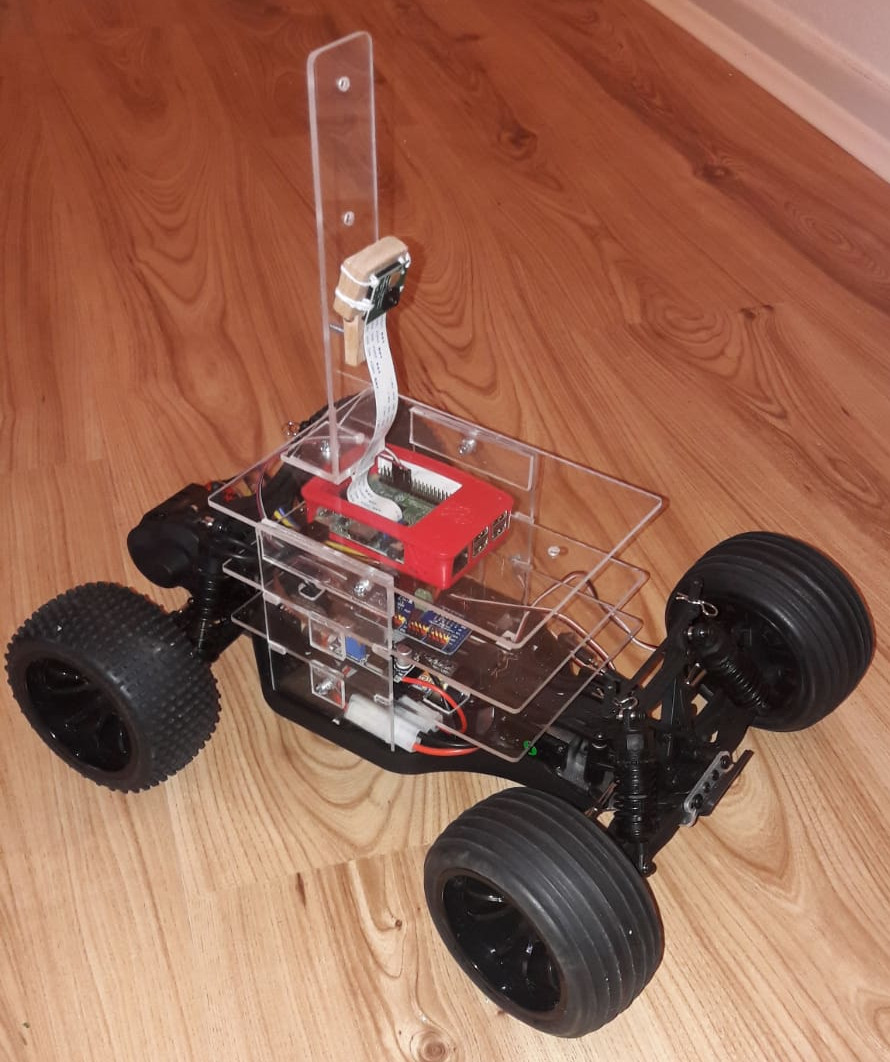
\includegraphics[width=0.6\linewidth]{images/hw_setup.jpg}
      \caption{RC Chassis mit Aufbau}
      \label{fig:img-hw-05}
    \end{minipage}
    \vspace{1cm}

  \subsection{Aufbau}
    % image of the exact setup
    \begin{minipage}{\columnwidth}
      \makeatletter
      \def\@captype{figure}
      \makeatother
      \centering
      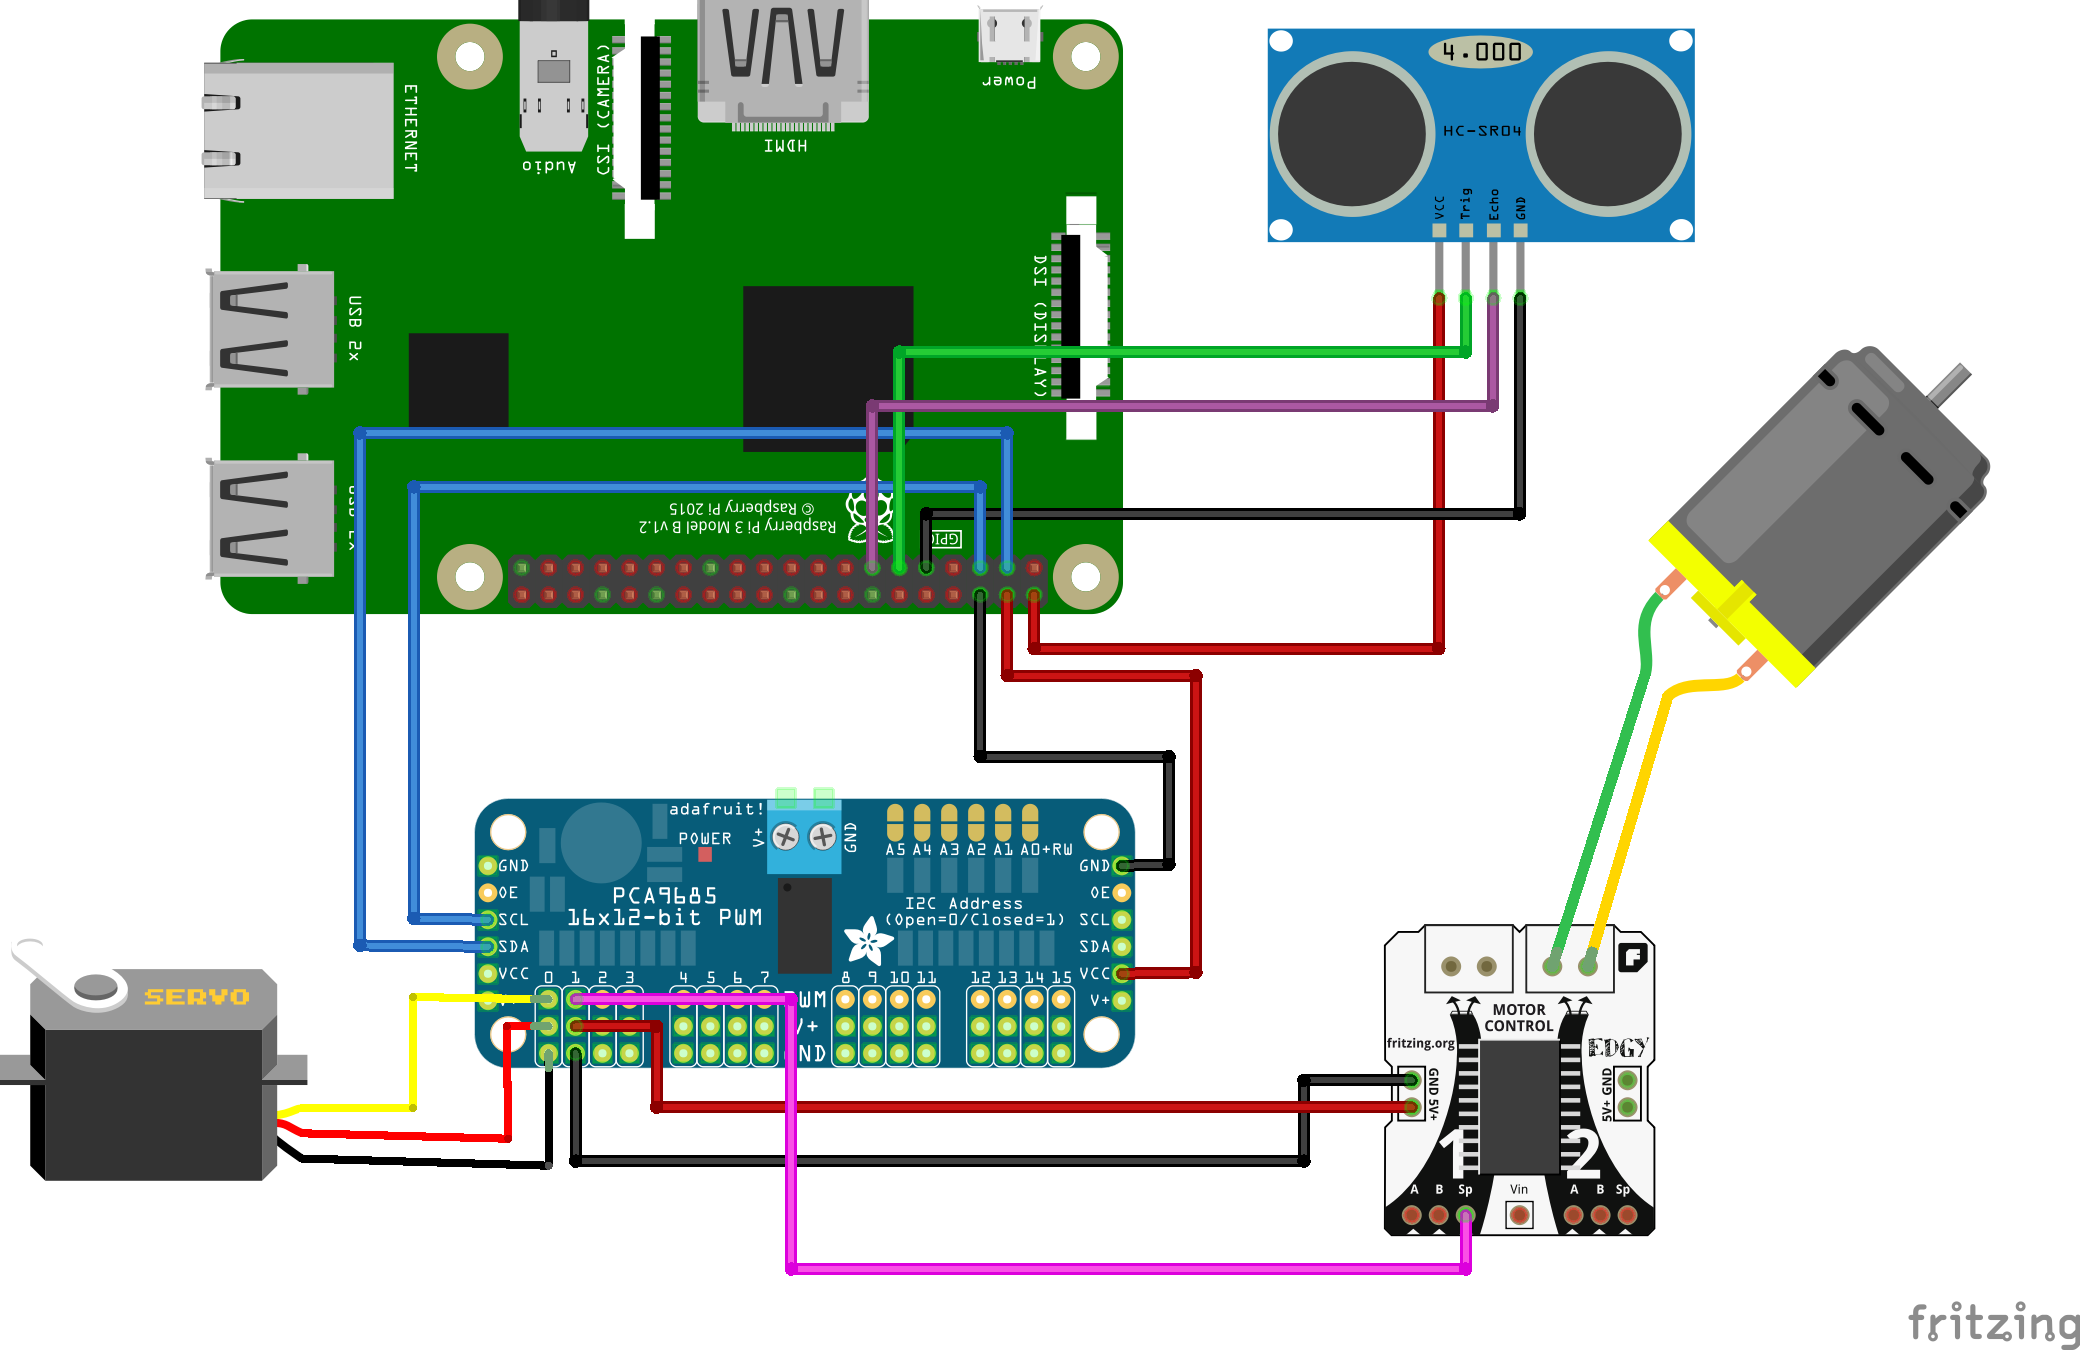
\includegraphics[width=1\linewidth]{images/hw_schematics.png}
      \caption{Schaltplan der Module}
      \label{fig:img-hw-06}
    \end{minipage}
    \vspace{1cm}

    \noindent
    Statt des EDGY Motor Control Moduls kommt in diesem Projekt der im RC
    Fahrzeug enthaltene Reely Fahrtenregler zum Einsatz. Die Anschlussbelegung
    ist weitesgehend dieselbe. \\

    \begin{minipage}{\columnwidth}
      \makeatletter
      \def\@captype{table}
      \makeatother
      \centering
      %\rowcolors{1}{grey}{white}
      \begin{tabular}{l | l | l | l}
      % \multicolumn{2}{|c}{Frame \#} & \multicolumn{4}{|c}{LCD 0/3} &
      GPIO Raspberry Pi & Modul & Pin & Beschreibung \\ \hline \hline
      2 / 5V & SR-04 & VCC & Spannungsversorgung \\
      3 / GPIO 2 & PCA9685 & SDA & I2C Datenleitung PWM Modul \\
      4 / 5V & PCA9685 & VCC & Spannungsversorgung PWM Modul \\
      5 / GPIO 3 & PCA9685 & SCL & I2C Taktsignal PWM Modul \\
      6 / GND & PCA9685 & GND & Masse PWM Modul \\
      9 / GND & SR-04 & GND & Masse Ultraschallsensor \\
      11 / GPIO 17 & SR-04 & TRIG & Trigger Impuls \\
      13 / GPIO 27 & SR-04 & TRIG & Echo \\
      
      \end{tabular}
      \caption{Pinbelegung}
      \label{tab:hw-01}
    \end{minipage}

